\section{Study 1: calibration-marginal versus plug-in adaptive testing}
\label{sec:study1}

\paragraph{Frozen decisions.} Table~\ref{tab:confirm} reports the four contrasts at $N=8$ as
the relative improvement of EOST-M over the baseline of each hypothesis (log loss for H1 and
H2, score error for H3, $|\mathrm{coverage}-0.9|$ for H4); an asterisk marks a
Holm-significant difference, and none favoured a baseline. \textbf{H2 is \DecHTwo}: EOST-M
lowered the held-out log loss on \PosHTwo\ of \NBHTwo\ benchmarks (median \MedImpHTwo\%),
significantly on \FavHTwo; the median gain was \MedImpHTwoNfour\% at $N=4$ and only
\MedImpHTwoNsixtyfour\% at $N=64$. \textbf{H3 is \DecHThree}: the score error fell by a
median of \MedImpHThree\% relative to naive subsampling (\FavHThree\ benchmarks
significant). \textbf{H4 is \DecHFour}: EOST-M reduced the miscalibration of plug-in
Fisher CAT by a median of \MedImpHFour\% (\FavHFour\ significant). \textbf{H1 is
\DecHOne}: EIG beat entropy on \PosHOne\ of \NBHOne\ benchmarks, but by a median of only
\MedImpHOne\% and significantly on \FavHOne, short of the threshold; the sign predicted by
the EOST thesis holds at every panel size, but its size on held-out prediction is small once
calibration uncertainty is integrated (Corollary~\ref{cor:blind}). On GSM8K, H2--H4 point
the same way without significance; its leaderboard spans the whole accuracy range, so an
eight-system panel leaves the fewest items unlocated (\GsmFracExtremeNeight\% against a median
of \OtherFracExtremeNeight\% elsewhere).

\begin{table}[htbp]
\centering\footnotesize
\caption{Study 1: relative improvement (\%) of EOST-M for H1--H4 at $N=8$.}
\label{tab:confirm}
\setlength{\tabcolsep}{5pt}
\begin{tabular}{@{}lrcccc@{}}
\toprule
 & & H1 & H2 & H3 & H4 \\
Benchmark & targets & vs Entropy:mg & vs MFI:pi & vs Naive & vs MFI:pi \\
\midrule
GSM8K & 60 & $+2.7$* & $+2.4$ & $+16.8$ & $+11.6$ \\
ARC-C & 60 & $+0.4$ & $+4.7$* & $+61.0$* & $+41.6$* \\
HellaSwag & 60 & $+5.5$* & $+9.6$* & $+68.4$* & $+46.8$* \\
WinoGrande & 60 & $+3.1$* & $+4.9$* & $+53.4$* & $+57.3$* \\
MMLU & 60 & $+2.9$* & $+5.0$* & $+55.3$* & $+59.0$* \\
SWE-bench V. & 60 & $+0.7$ & $+6.1$* & $+46.9$* & $+31.7$* \\
LiveCodeBench & 28 & $+1.0$ & $+6.4$* & $+51.3$* & $+48.1$* \\
CRUXEval-O & 31 & $+0.5$ & $+5.4$* & $+57.7$* & $+33.4$* \\
\midrule
decision & & 4/0 not supported & 7/0 supported & 7/0 supported & 7/0 supported \\
\bottomrule
\end{tabular}
\end{table}


\paragraph{Dependent targets.} Many Open LLM Leaderboard systems are fine-tunes or merges of
a few base models. Re-analysed post hoc with heuristic families as units, the frozen
decisions are unchanged. With strict clusters (\CluStrictUnitsMin\ to \CluStrictUnitsMax\
units per benchmark), H3 and H4 remain supported, but H2 is significant on only
\CluHTwoStrFav\ benchmarks, below the threshold, although its median effect is unchanged
(\CluHTwoStrMed\%, 95\% cluster-bootstrap interval \CluHTwoCILo--\CluHTwoCIHi\%). The
predictive gain is therefore not in doubt, but its significance with targets as units
overstates the evidence; study~2 was designed with one target per cluster to settle this.

\paragraph{Where the gain comes from.} EOST-M differs from plug-in Fisher CAT in its
criterion and in its measurement model, and Table~\ref{tab:factorial} crosses the two. At
$N=8$, replacing plug-in parameters by expected response functions improves held-out log
loss by a median of \FactEntMgLL\% even with entropy selection, whereas changing the
criterion under plug-in parameters changes little (\FactEntPiLL\% for entropy,
\FactEigPiLL\% for EIG); combining both gives \FactEigMgLL\%. For the score the criterion
matters more: entropy is the worst adaptive rule under both models (\FactEntMgIAE\% under
the marginal model), whereas EIG:mg improves the score IAE by \FactEigMgIAE\%. Under the
marginal model the four information criteria (MFI, PWFI, EIG, EVR) are practically
indistinguishable---their mean log losses differ by at most \InfoSpreadLL\% and their score
errors by at most \InfoSpreadIAE\%---as the first-order equivalence of
Proposition~\ref{prop:local} predicts. Most of the gain thus comes from integrating
calibration uncertainty, and EIG is the principled member of an equivalence class rather
than a uniquely better rule.

\begin{table}[htbp]
\centering\footnotesize
\caption{Study 1: gain over MFI:pi by criterion and measurement model (median, \%).}
\label{tab:factorial}
\setlength{\tabcolsep}{3.5pt}
\begin{tabular}{@{}rrrrrrrrrr@{}}
\toprule
 & & \multicolumn{4}{c}{holdout log loss} & \multicolumn{4}{c}{score IAE} \\
\cmidrule(lr){3-6}\cmidrule(lr){7-10}
$N$ & $B$ & Ent:pi & EIG:pi & Ent:mg & EIG:mg & Ent:pi & EIG:pi & Ent:mg & EIG:mg \\
\midrule
4 & 8 & $-0.8$ & $-0.1$ & $+5.0$ & $+7.1$ & $-12.3$ & $-0.8$ & $-15.2$ & $+11.7$ \\
8 & 8 & $-1.8$ & $0.0$ & $+4.4$ & $+5.2$ & $-17.5$ & $+0.7$ & $-9.2$ & $+7.5$ \\
16 & 8 & $-1.4$ & $0.0$ & $+2.0$ & $+3.6$ & $-18.7$ & $-0.7$ & $-10.9$ & $+5.9$ \\
32 & 6 & $-1.8$ & $0.0$ & $-0.5$ & $+1.9$ & $-23.4$ & $+0.2$ & $-22.8$ & $+7.4$ \\
64 & 6 & $-2.0$ & $+0.1$ & $-1.3$ & $+1.1$ & $-17.5$ & $+0.6$ & $-16.7$ & $+6.6$ \\
\bottomrule
\end{tabular}
\end{table}


The gain over plug-in Fisher CAT decreases monotonically with the panel size on every
benchmark (Figure~\ref{fig:heatmap}, panel a, where an asterisk marks a Holm-adjusted
$p<0.05$), as Proposition~\ref{prop:cap} predicts, since the uncertainty of item difficulties
shrinks as calibrators are added; panel~b gives the score error and panel~c the contrast with
entropy (H1). Calibration diagnostics show the mechanism. With four calibrators
\FracExtremeNfour\% of the items were answered identically by every calibrator
(\FracExtremeNsixtyfour\% with 64), so their difficulty is located only by the prior. Under
the empirical-Bayes prior, plug-in discriminations above 4 are practically absent with small
panels (\FracAgtFourNfour\% of items at $N=4$, \FracAgtFourNsixtyfour\% at $N=64$), while the
expected response function shrinks the median effective discrimination from \AmapNfour\ to
\AeffNfour\ at $N=4$, as Proposition~\ref{prop:cap} prescribes. The
overconfidence of plug-in testing at small $N$ therefore comes mainly from treating poorly
located difficulties as known, and across benchmarks and panel sizes the log-loss gain of
EOST-M grows with the fraction of unlocated items (Spearman $\rho=\MechRho$, exploratory).

\begin{figure}[htbp]
\centering
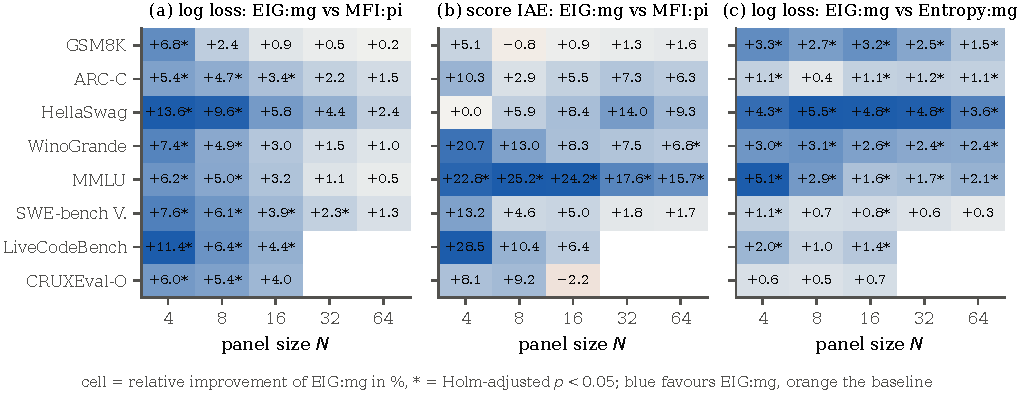
\includegraphics[width=0.92\linewidth]{figures/heatmap_improvement.pdf}
\caption{Study 1: relative improvement (\%) of EOST-M by benchmark and panel size.}
\label{fig:heatmap}
\end{figure}

\paragraph{Learning curves and efficiency.} Every model-based policy starts below the naive
estimator, because the calibrated model predicts the bank before any item is asked
(Figure~\ref{fig:curves-err}). Plug-in policies reduce the error fastest in the first items
(at $t=5$ a plug-in policy is ahead of EOST-M on \EarlyPluginBetter\ of \NCurveBanks\
benchmarks) but then level off: between $t=25$ and $t=100$ the error of plug-in Fisher CAT
falls by a median of \PlateauPi\%, that of EOST-M by \PlateauMg\%, and after 100 items
EOST-M is ahead on \FinalEigBelowMfi\ of \NCurveBanks\ benchmarks---the signature of a bias
floor inherited from the plug-in parameters. At $N=8$, EOST-M matched the score error of 100
uniformly sampled items after a median of \EffItemsMedianNeight\ items (between
\EffItemsMinNeight\ and \EffItemsMaxNeight\ across benchmarks), and after \EffItemsMedianNmax\
with the largest panels. Adaptivity itself contributes: random items scored by the same
marginal model had a mean score IAE of \IAErandmgNeight\ against \IAEeigmgNeight\ for
EOST-M, whose error was significantly lower on \RandIaeFav\ of \RandIaeNB\ benchmarks. Late
in the test, entropy selection under the marginal model catches up, and the crossover comes
later on larger banks (Spearman $\rho=\CrossRho$ over \CrossPoints\ benchmark--panel
combinations, exploratory), the regime change described by Proposition~\ref{prop:evr}; the
score-targeted criterion moved in the predicted direction, but only part of the way. Short
adaptive tests also rank systems well: after 25 items, Kendall's $\tau$ with the true accuracy
had a median of \TauEigTwentyfive\ for EOST-M, \TauMfiTwentyfive\ for plug-in Fisher CAT and
\TauNaiveTwentyfive\ for random items (exploratory).

\begin{figure}[htbp]
\centering
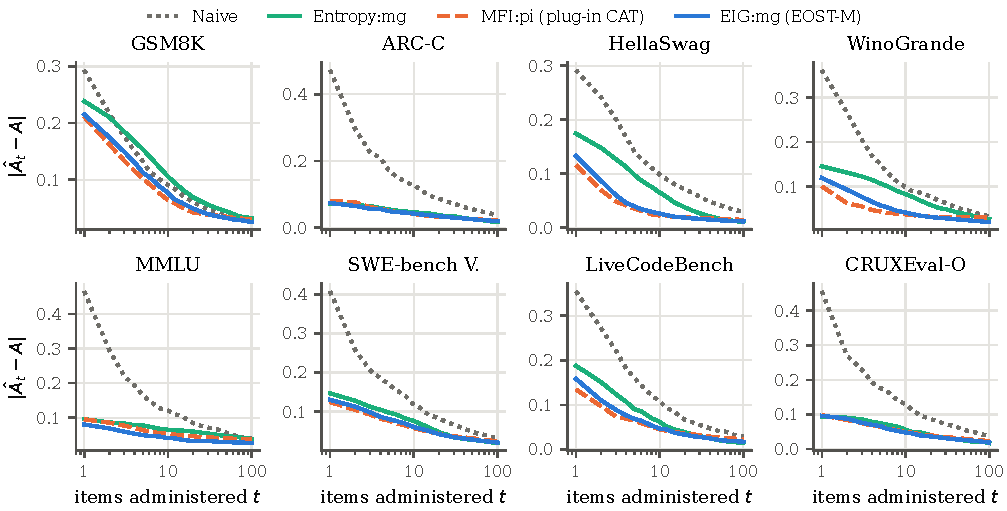
\includegraphics[width=\linewidth]{figures/curves_err_N8.pdf}
\caption{Study 1: absolute score error as items are administered ($N=8$).}
\label{fig:curves-err}
\end{figure}

\paragraph{Uncertainty.} Plug-in posteriors are overconfident (Figure~\ref{fig:coverage}a):
at $N=8$ the 90\% interval of plug-in Fisher CAT covered the score \CovMfipi\ of the time,
EOST-M's \CovEigmg\ and Naive's model-free Wilson interval \CovNaive. Marginalization
removes much of the overconfidence, but no model-based adaptive policy reaches nominal
coverage on real data. On the synthetic banks (Figure~\ref{fig:coverage}b), EOST-M's
coverage at $N=8$ is \SynTwoplEigMgCovNeight\ when the model is well specified,
\SynGuessEigMgCovNeight\ with guessing and \SynTwodimEigMgCovNeight\ with a second ability
dimension, and as the panel grows coverage rises towards the nominal level on synthetic data
but falls on real data: more calibrators sharpen the item posteriors, which helps when the
model is adequate and exposes its misfit when it is not. With known abilities, EOST-M also
had the smallest ability error at $N=8$ on all three synthetic banks
(\SynTwoplEigMgErrNeight, \SynGuessEigMgErrNeight\ and \SynTwodimEigMgErrNeight, against
\SynTwoplMfiPiErrNeight, \SynGuessMfiPiErrNeight\ and \SynTwodimMfiPiErrNeight\ for plug-in
Fisher CAT).

\begin{figure}[htbp]
\centering
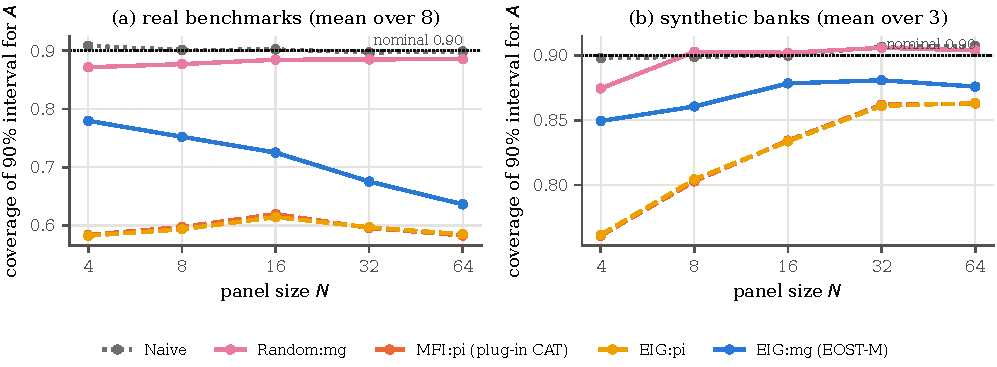
\includegraphics[width=0.88\linewidth]{figures/coverage.pdf}
\caption{Study 1: coverage of the 90\% score interval as a function of the panel size.}
\label{fig:coverage}
\end{figure}

\paragraph{Sensitivity and post hoc probes.} Removing near-duplicate calibrators leaves the
H2 gain essentially unchanged (\SensDedupHTwoNeight\% against
\SensMainDedupBanksHTwoNeight\% on the same benchmarks), but the empirical-Bayes hyperprior
is essential: with a fixed weakly-informative prior the H2 gain falls to
\SensFixedpriorHTwoNeight\% (main analysis: \SensMainHTwoNeight\%), because for an item
that the panel cannot locate the expected response function is essentially the prior
predictive. The one-parameter variant of the frozen plan is degenerate---its likelihood is
invariant to a joint rescaling, and its mode inflates the common discrimination (median
\OneplMedianA)---and is not interpreted. A post hoc variant with
$\log a\sim\mathcal N(0,0.05^2)$ confirms Corollary~\ref{cor:blind}: with one common
discrimination the EIG--entropy difference is \SensOneplregHOneNeight\% under the marginal
model and \SensOneplregHOnePiNeight\% under plug-in parameters, against
\SensMainHOneNeight\% and \SensMainHOnePiNeight\% with item-specific discriminations.

Three post hoc probes, with decision rules recorded before running, then tested a competing
explanation of H2. (i) Posterior-mean plug-in parameters are no remedy (log loss
\PhMfieapLLNeightAbs\% worse than EOST-M), but a regularized Rasch-type plug-in test is a
strong baseline: EOST-M's log loss was lower on all \PhMfioneprLLNeightB\ benchmarks, yet only
by a median of \PhMfioneprLLNeightAbs\% (significant on \PhMfioneprLLNeightFav), and the
Rasch-type intervals were better calibrated (coverage \PhCovMfionepr\ against \PhCovEigmg);
averaging Fisher information over the item posterior selected items as well as EIG (median
difference \PhEfiLLNeightAbs\%), so the optimism of Corollary~\ref{cor:jensen} did not
matter. (ii) Shrinking EOST-M's discriminations towards a common value did not combine the
two remedies: no setting met the criterion fixed in advance (coverage between \ShrMgCovMin\
and \ShrMgCovMax). (iii) The Rasch-type intervals were wider on all \PhThreeWiderBanks\
benchmarks without more accurate estimates, and across all cells coverage was almost a
monotone function of the ratio of interval width to score error (Spearman $\rho=\PhThreeRho$),
a ratio below that of a calibrated Gaussian interval in every cell. The constrained model is
better calibrated because it is less confident, and since random items under the same model
cover \CovRandmg\ of the time, the shortfall arises when adaptive selection meets a
misspecified model. Study~2 tests the Rasch-type competitor under a frozen plan.
